\section{Drift Chamber System Conceptual Design}

When the CLAS detector was upgraded to become the CLAS12 detector, the
drift chambers were re-designed.  We kept many of the design concepts
of the original CLAS chambers, but made improvements in a number
of areas.

\subsection{Physics Requirements for {\tt CLAS12} Forward Tracking}

There are several broad areas of physics research that drive 
the design of the forward tracking system: 
spectroscopic studies of excited baryons, investigations of 
the influence of nuclear matter on propagating quarks, studies of polarized 
and unpolarized quark distributions, and a comprehensive measurement of 
generalized parton distributions (GPDs). 

The cross sections for these processes are small, necessitating high-luminosity 
experiments.  A variety of simulated experiments rely on luminosities of 
10$^{35}$~cm$^{-2}$s$^{-1}$ to achieve the desired statistical accuracy in 
runs of a few months duration.  This is an order of magnitude increase
compared to the previous CLAS detector.  

The new kinematic range available to the CLAS12 experiment is
characterized not only by smaller cross sections, but also by more outgoing 
particles per event, with those particles being emitted at larger momenta
and smaller laboratory angles.  
A final state of a few high-momentum, forward-going particles (the electron as well as one 
or more mesons), combined with a moderate-momentum baryon emitted at large 
angles, is the typical event type that determines the specifications of the 
tracking system. 

To cover as much of the hadronic center-of-mass region as possible, the forward 
detector must provide tracking for charged particles emitted at polar angles 
from 5$^\circ$ to 40$^\circ$.  This is complemented by the angular coverage of
the central tracking system which covers polar angles from  35$^\circ$ to approximately 120$^\circ$.

In addition to large acceptance, our experimental program requires
small systematic errors.  To measure our electroproduction cross-sections
to an accuracy of a few percent, we must know the scattered electron's
momentum to $1\%$ and its angle to 1 mrad.  
We require even better momentum resolution on the scattered
electron (with momentum up to 10 GeV/c) to be able to identify particles
by missing mass, an important technique in exclusive reaction studies.
This requirement to identify one (and only one) missing particle led to our 
most stringent design specification on the fractional momentum resolution:
$dp/p = 0.3\%$ for electrons emitted at small angles ($7^{\circ}$) and high
momentum (10 GeV/c).  

Table~\ref{fwd-dc-physics-specifications} lists the physics goals for the CLAS12 program
main and the resulting design specifications that will allow us to achieve these goals.


%%%%%%%%%%%%%%%%%%%%%%%%%%%%%%%%%%%%%%%%%%%%%%%%%%%%%%%%%%%%%%%%%%%%%%%%%
\small{
\begin{table}[ht]
\begin{center}
\begin{tabular}{||c|c|c||} \hline \hline
   {\bf Goal}         & {\bf Physics Specification} & {\bf Design Specification}\\ \hline
Measure $\Gamma_v$  & $d \theta <$ 1mrad   & planar chambers \\ 
accurately  & sin$\theta ~d \phi < $1 mrad & $+/- 6^\circ$ stereo angle   \\ 
  & $dp/p < 1\% $ & identical cells (each superlayer)  \\ \hline
Select exclusive reaction; &    & $250~\mu$m  accuracy per cell\\ 
only one missing particle    & $dp/p < 0.3\%$ at 10 GeV/c &    chamber alignment $<100\mu$m\\  \hline
Small       & Luminosity = $10^{35}$~cm$^{-2}$s$^{-1}$  & six 6-layer superlayers \\ 
cross sections  & high efficiency & $> 95\%$ layer efficiency \\ \hline
large acceptance   & $\delta\phi = 50\%$ at $5^\circ$ & thin endplates\\ \hline
\end{tabular}
\caption{\small{\bf Physics goals and the resulting physics and design specifications.}}
\label{fwd-dc-physics-specifications}
\end{center}
\end{table}
}
%%%%%%%%%%%%%%%%%%%%%%%%%%%%%%%%%%%%%%%%%%%%%%%%%%%%%%%%%%%%%%%%%%%%%%%%%

\subsection{Drift Chamber Conceptual Design}

The overall tracking requirements:
\begin{itemize}
\item $0.3\%$ fractional momentum resolution at $7^{\circ}$ and 10~GeV/c, and 
\item efficient tracking at a luminosity of 
10$^{35}$~cm$^{-2}$s$^{-1}$
\item large angular acceptance 
\end{itemize}
are the main drivers for the drift chamber design.  

Because the previous {\tt CLAS} drift chamber system~\cite{dcnim} operated 
successfully for 8~years, we re-used many of the design concepts and 
most of the utility infrastructure, including
parts of the gas mixing and handling system, the high-voltage 
and low-voltage systems, and many of the high voltage and signal cables. 
Refer to our 
article on the previous {\tt CLAS} detector~\cite{clasnim} and our article 
on the previous drift chambers themselves~\cite{dcnim} for details of the 
previous detector and chambers.  

We kept the same chamber layout as in {\tt CLAS}:
the forward tracking system consists of three regions divided into six
sectors as shown in Fig.~\ref{chambers-and-torus}; located just before, inside, 
and just outside the torus field volume, named Regions~1, 2, 
and 3 (and referred to as R1, R2 and R3), respectively.  
Each chamber has its wires arranged in two superlayers (SL) of
six layers each, with the wires in the two superlayers strung with 
$\pm$6$^\circ$ stereo angles, respectively.  The cell structure is 
hexagonal, that is, each sense wire is surrounded by six field wires.  This 
arrangement offers good 
resolution with very good pattern recognition properties.  

The major difference compared to the previous design is that the 
chambers are located further downstream from the target and thus the drift
cells cover a smaller solid angle than those in the previous {\tt CLAS} 
chambers, allowing efficient tracking at higher luminosities because the 
accidental occupancy from particles not associated with the event is smaller.  

\subsection{Design Features}

Table~\ref{fwd-dc-design-parms} lists the main design parameters for each 
region of the {\tt CLAS12} drift chambers.  For the purposes of simulating 
track resolutions, we assumed that the position resolution of the individual 
drift cells would be 250~$\mu$m.  

%%%%%%%%%%%%%%%%%%%%%%%%%%%%%%%%%%%%%%%%%%%%%%%%%%%%%%%%%%%%%%%%%%%%%%%%%
\small{
\begin{table}[hbt]
\begin{center}
\begin{tabular}{||c|c|c|c||} \hline \hline
            &{\bf Region 1}&{\bf Region 2}&{\bf Region 3}\\ \hline
Distance from target & 2.3 m    & 3.5 m        & 4.9 m    \\ \hline
Num. of superlayers  & 2        & 2            & 2        \\ \hline
Layers/superlayer    & 6        & 6            & 6        \\ \hline
Wires/layer          & 112      & 112          & 112      \\ \hline
Cell radius (each SL) & 0.78, 0.81 cm  & 1.14, 1.32 cm      & 1.87, 1.96 cm  \\ \hline
Active time window   & 150 ns   & 325 - 1000 ns & 750 ns   \\ \hline
\end{tabular}
\caption{\small{Design parameters for the {\tt CLAS12} drift chambers.}}
\label{fwd-dc-design-parms}
\end{center}
\end{table}
}
%%%%%%%%%%%%%%%%%%%%%%%%%%%%%%%%%%%%%%%%%%%%%%%%%%%%%%%%%%%%%%%%%%%%%%%%%

\subsubsection{Design Elements in Common with the Previous CLAS Chambers}
The CLAS12 drift chambers share some design characteristics with the
previous CLAS chambers:
\begin{itemize}
\item {\bf Wire Layout}
\begin{itemize}
\item ``brick-wall'' wire layout resulting in individual hexagonally-shaped
drift cells in a plane perpendicular to the wire direction
\item sense wire layers are grouped into two ``superlayers'' of 6 layers each
\item the ``endplates'' on the two sides of the chamber are tilted 
at approximately 60 deg. with respect to each other
\end{itemize}
\item {\bf Chamber Body Design}
\begin{itemize}
\item to maximize the active volume of the chamber, the ``dead areas'', e.g.
the endplates and electronics boards are kept as thin as possible
\item because of the possibility of large eddy currents and resultant
force on the endplates in case of the quench of our torus magnet, we
use non-conducting G10 endplates for our R2 chambers
\end{itemize}
\item {\bf Gas Choice:} 90:10 Argon:CO$_2$ mixture.  We operate at a gas gain of 
about $5 \times 10^4$.
\end{itemize}


\subsubsection{Design Improvements Compared to the Previous CLAS Chambers}
To improve the chambers' peformance we made some important changes to the design:
\begin{itemize}
\item {\bf Mechanical Design}
\begin{itemize}
\item all chambers have the same, roughly equilateral triangular, shape
\item the previous CLAS chambers were interconnected to each other (R1) or 
connected directly to the torus (R2).  In the present chambers all of the wire tension
is borne by the endplates and thus they can be independently mounted.
The key to this improvement is the use of  
ultra-stiff endplate assemblies that obtain their stiffness 
by a flanged design
\item all chambers are independent and self-supporting, allowing easy
maintenance and repair.  The chambers are attached to the torus cryostat using 6 independent
rods with ``ball and socket'' ends, meaning that the chambers can be
moved out to maintenance position and moved back to the operating 
postion by turning one precision turn-buckle assembly
\end{itemize}
\item {\bf Cell Design and Wire Layout}
\begin{itemize}  
\item For the previous CLAS detector, the $\phi$ resolution times $\sin \theta$ was about two 
times larger than the $\theta$ resolution.  To have more equal resolution in 
the two angles, we doubled our stereo angle from 0 and 6$^\circ$ to 
$\pm$6$^\circ$
\item all chambers are planar, with the first ``superlayer'' (of 6 layers)
tilted at a 6$^\circ$ stereo angle, and the second superlayer at a -6$^\circ$ stereo
angle
\item all wires within one superlayer are parallel to each other, thus
every cell in the superlayer is identical, making it easier to model
and fit the distance to time response
\end{itemize}
\item {\bf Wire Choice}
\begin{itemize}
\item all chambers are strung with 30 $\mu m$ gold-plated Tungsten wire,
considerably tougher and easier to handle than our previous choice 
of 20 $\mu m$ wire
\item the choice of the cathode (``field'') wire is 80 $\mu m$ gold-plated
Cu-Be wire, tougher and with better surface properties than our previous
choice of 140 $\mu m$ gold-plated Aluminum wire
\item  Our choice of guard wire is 140 $\mu m$ diameter, gold-plated
copper-beryllium.  These wires were strong enough that we pre-tensioned 
the chambers using only the guard wires; a simplification in the process.
\end{itemize}
\end{itemize}



Table~\ref{fwd-dc-design-features} lists the advantages and disadvantages
of various design features.
%%%%%%%%%%%%%%%%%%%%%%%%%%%%%%%%%%%%%%%%%%%%%%%%%%%%%%%%%%%%%%%%%%%%%%%%%
\begin{table}[ht]
\begin{center}
\begin{tabular} {||c|c|c||} \hline \hline
{\bf Design Feature  }       &{\bf Advantages} &{\bf Disadvantages}\\ \hline
``All-wire design'' & Little cathode emission & \\ \hline
Small Cells & Robust track-finding  & Many wires to string \\ \hline
Hexagonal Cells & Minimum number of wires  & Angle-dependence of time to distance  \\ \hline
30 $\mu m$ diameter sense wire & Resistant to wire breakage & Higher operating voltage \\ \hline
80 $\mu m$ diameter field wire & Lower total wire tension & Higher fields on cathode wires \\ \hline
Opposite voltage  & Identical fields & More HV \\
for sense and field & for all layers & channels required \\ \hline
Self-supporting design & Easier maintenance & 1 - 2 mm bowing of endplates \\ \hline
\end{tabular}
\caption{\small{Design features of the {\tt CLAS12} drift chambers.}}
\label{fwd-dc-design-features}
\end{center}
\end{table}
%%%%%%%%%%%%%%%%%%%%%%%%%%%%%%%%%%%%%%%%%%%%%%%%%%%%%%%%%%%%%%%%%%%%%%%%%

%%%%%%%%%%%%%%%%%%%%%%%%%%%%%%%%%%%%%%%%%%%%%%%%%%%%%%%%%%%%%%%%%%%%%%%%%%%
%\begin{figure}[htbp]
%\vspace{14.0cm}
%\special{psfile=img/garfield1.eps hscale=30 vscale=27 hoffset=40 voffset=165}
%\special{psfile=img/garfield2.eps hscale=30 vscale=27 hoffset=40 voffset=-5}
%\special{psfile=img/garfield3.eps hscale=30 vscale=27 hoffset=230 voffset=165}
%\special{psfile=img/garfield4.eps hscale=30 vscale=27 hoffset=230 voffset=-5}
%\caption{\small{GARFIELD calculations of the electric field lines (top)
%and drift time vs. drift distance (bottom) for a Region~3 drift cell.  The 
%left plots show the configuration with a 20-$\mu$m diameter sense wire and 
%the right plots show the configuration with a 30-$\mu$m diameter sense wire.
%The high voltages were set to provide the same gas gain for each
%configuration.}}
%\label{garfield-20-vs-30-micron}
%\end{figure}
%%%%%%%%%%%%%%%%%%%%%%%%%%%%%%%%%%%%%%%%%%%%%%%%%%%%%%%%%%%%%%%%%%%%%%%%%%%


\subsubsection{Wire Diameter}
One of the most significant design changes was the decision 
to use 30-$\mu$m diameter sense wire rather than the previously-used 
20~$\mu$m wire. 
This should make the chambers more resistant to wire 
breakage.  The larger radius of the sense wires means that higher 
voltages will be required to achieve the same gas gain, see Section \ref{determine-operating-parameters}
for more details.
Prototypes were built to study possible negative side-effects of the 
higher voltage operation, such as leakage currents on the circuit boards 
and/or higher rates of cathode emission from the field wire surfaces.
No such effects were seen.
We discuss the wire choice in more detail in section~\ref{construction}.

%In addition to being tougher than 20-$\mu$m wire, the higher voltages 
%(~ 250 V higher)
%required for 30-$\mu$m wire to achieve the same gain will result in
%higher and more constant drift velocities.
%Fig.~\ref{garfield-20-vs-30-micron} shows GARFIELD calculations for a Region~3 drift cell
%with both a 20-$\mu$m and a 30-$\mu$m diameter sense wire.  Here the
%cells with the thicker sense wire will have a significantly higher drift 
%velocity, which reduces the time window, and hence the 
%chamber occupancy.





%%%%%%%%%%%%%%%%%%%%%% Figure : garfield-20-30-micron %%%%%%%%%%%%%%%%%%%%%%
%\begin{figure}
%\vspace{4.5cm}
%\begin{picture}(50,50)
%\put(-10,10)
%{\hbox{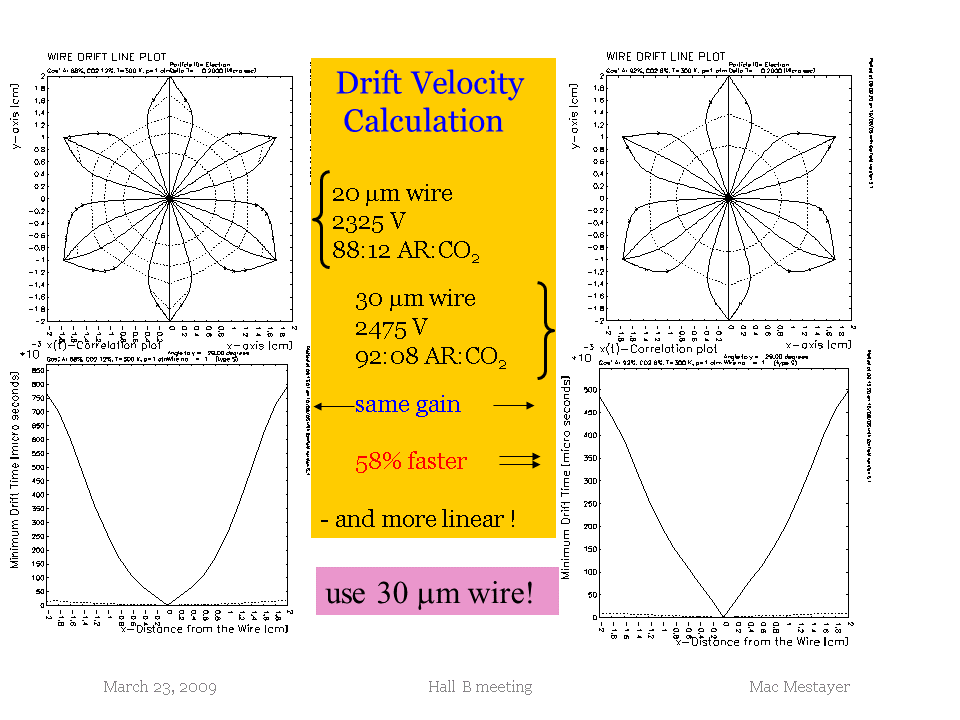
\includegraphics[width=0.5\columnwidth,natwidth=610,natheight=642]{garfield-20-30-micron.png}}}
%\end{picture}
%\caption{\small{Plots of field lines and isochrones (top) or drift time vs.
%distance (bottom).  Calculations are for 20 $\mu m$ wire (left) or 30 $\mu m$ (right).}}
%\end{figure}   
%%%%%%%%%%%%%%%%%%%%%%%%%%%%%%%%%%%%%%%%%%%%%%%%%%%%%%%%%%%%%%%%%%%%%%%%%%


 
